\section*{Exercice 189 -- Modélisation}
\setcounter{exo}{0}
%CCS PSI 2009

\subsection*{Modélisation du comportement d’un couple d’électro-aimants}
L'étude porte sur un seul couple d'électro-aimants. 
\begin{center}
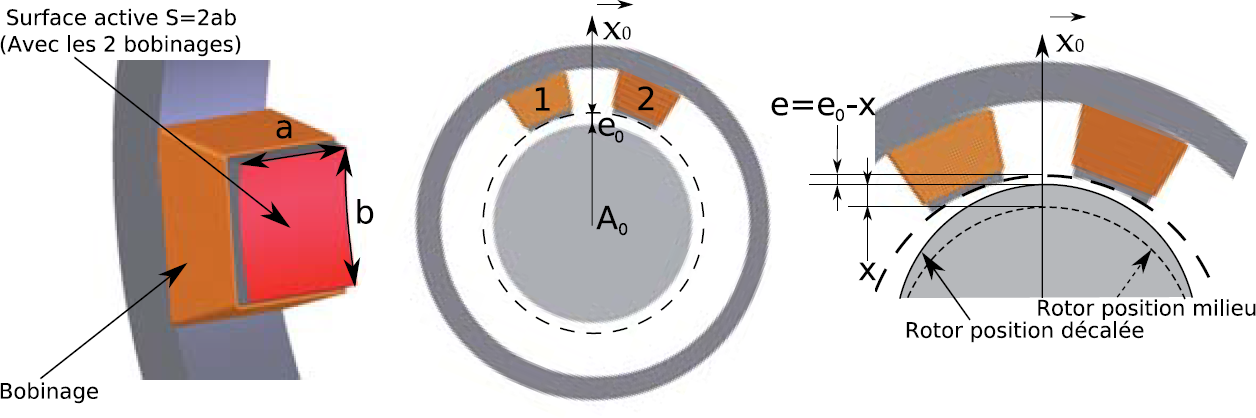
\includegraphics[width=\linewidth]{990_01}
\end{center}

Lorsque le bobinage, enroulé autour de fines plaques en fer doux, est alimenté
par un courant $I$, un champ magnétique $B$ apparaît dans l'entrefer entre
l'électro-aimant et le rotor, tel que $N\cdot I =\dfrac{2e}{\mu_0 }B$.

Ce champ magnétique permet de créer un effort exercé par l'électro-aimant sur
le rotor, dans l'axe de l'électro-aimant, tel que $F=\dfrac{B^2 S}{2\mu_0}$ où $S=ab$ est la surface active du couple d'électro-aimants.


\subsubsection*{Spécifications de fonctionnement}
\begin{itemize}
\item L'échauffement maximal des bobinages impose une intensité maximale telle que $I_{\text{max}}=\SI{5}{A}$.
\item Le champ magnétique maximal dans un matériau ferro-magnétique est limité à $B_{\text{max}}=\SI{1,8}{T}$.
\end{itemize}

Données numériques :
\begin{itemize}
\item nombre de spires : $N=\SI{200}{spires}$;
\item perméabilité magnétique du vide $\mu_0 = 4\pi\times\SI{e-7}{H.m^{-1}}$;
\item valeur moyenne $e_0$ de l'entrefer $e_0=\SI{0,2}{mm}$;
\item diamètre de l'arbre $d=\SI{50}{mm}$;
\item surface active $S=\SI{300}{mm^2}$.
\end{itemize}


On note $\vect{F}=F\vect{x_0}$ l'effort exercé par le couple des électro-aimants sur le rotor
selon $\vect{x_0}$.

\subparagraph{}
\textit{Montrer que le couple des deux électro-aimants permet d'assurer l'effort
maximal transmissible tout en respectant les spécifications de fonctionnement.}
\ifprof
\begin{corrige}
\end{corrige}
\else
\fi

Un déplacement $x$, tel que $\vect{A_0A}=x\vect{x_0}$, de l'arbre par rapport au stator conduit
à une modification de l'effort exercé $F$. On note $e_0$ l'entrefer initial pour $x=0$ tel que $e=e_0-x$.

\subparagraph{}
\textit{Déterminer l'expression de l'effort $F$ en fonction de $x$, de $I$ et de paramètres
géométriques. Peut-on exercer un effort $\vect{F}$ suivant $\vect{-x_0}$ en modifiant $I$ ou
$e$ ? Déterminer la valeur numérique de la constante $\gamma$ telle que $F=\gamma \dfrac{I^2}{e^2}$.}
\ifprof
\begin{corrige}
\end{corrige}
\else
\fi


\subsection*{Modélisation d'un palier magnétique actif}
Les couples d'électro-aimants sont associés par paires diamétralement opposées.
On ne s'intéresse ici qu'au contrôle de la position du rotor selon $\vect{x_0}$ réalisé
par les électro-aimants 1, 2, 5 et 6. Pour simplifier :
\begin{itemize}
\item le couple des électro-aimants 1 et 2 crée un effort de norme $F_1$ sur le rotor,
\item le couple des électro-aimants 5 et 6 crée un effort de norme $F_2$ sur le rotor.
\end{itemize}


\begin{center}
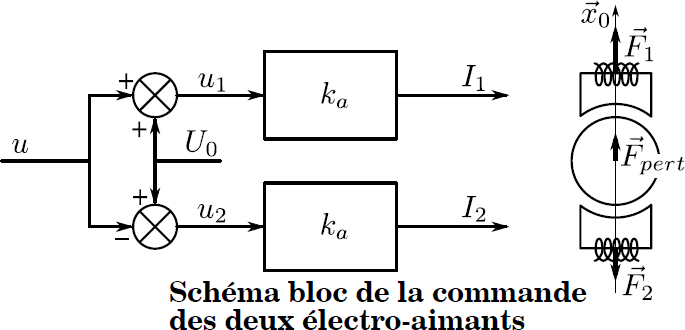
\includegraphics[width=\linewidth]{990_02}
\end{center}

On a :
\begin{itemize}
\item $\vect{F_1}=\left(F_0+\dd F_1\right) \vect{x_0}$;
\item $\vect{F_2}=-\left(F_0+\dd F_2\right) \vect{x_0}$;
\item $I_1 = I_0 +\dd I_1$;
\item $I_2 = I_0 +\dd I_2$;
\item $u = 0 +\dd u$;
\item $x = 0 +\dd x$.
\end{itemize}

Le point de fonctionnement de chaque couple d’électro-aimants est caractérisé
par $x=0$, $I=I_0$ et $F=F_0$ (voir figure 12). On admet que le comportement se
traduit par un effort dirigé de l'axe du rotor vers l'électro-aimant tel que $F_1 = \gamma \dfrac{I_1^2}{e_1^2}$ et $F_2=\gamma \dfrac{I_2^2}{e_2^2}$ avec $\gamma=2\times \SI{e-6}{Nm^2A^{-2}}$.

On note $\vect{F_{\text{pert}}} = F_{\text{pert}}\vect{x_0}$ un effort perturbateur s'exerçant sur le rotor.


\subparagraph{}
\textit{On note désormais $\vect{F_T}=F_t\vect{x_0}$ l'effort total exercé par les deux couples
d'électro-aimants. Montrer que l'expression linéarisée de $F_T$ peut s'écrire en
fonction de $u$ et $x$ sous la forme $F_T = \dfrac{4\gamma k_a^2 U_0^2}{e_0^2} \left(\dfrac{u}{U_0} + \dfrac{x}{e_0} \right)$.}
\ifprof
\begin{corrige}
\end{corrige}
\else
\fi


En première approximation, la masse $m=\SI{10}{kg}$ du rotor se répartit équitablement
au centre de chaque palier magnétique radial. Ceci revient à étudier le
comportement dynamique d'une masse ponctuelle (masse $m/2$) placée au centre
de chaque palier magnétique radial.

\subparagraph{}
\textit{Appliquer le Principe Fondamental de la Dynamique à la masse ponctuelle
(de masse $m/2$) et en déduire une relation entre $F_T$, $F_{\text{pert}}$ et $x$. Compléter
le schéma-blocs du palier magnétique ayant pour entrée la tension $u$ et pour sortie la position $x$, et faisant apparaître l'effort perturbateur $F_{\text{pert}}$.}
\ifprof
\begin{corrige}
\end{corrige}
\else
\fi


\begin{center}
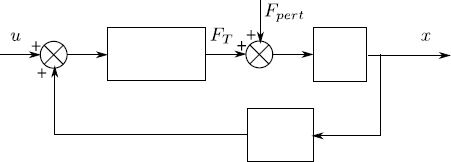
\includegraphics[width=\linewidth]{990_03}
\end{center}


\subparagraph{}
\textit{Déterminer la fonction de transfert $H_{\text{PM}}=\dfrac{X(p)}{U(p)}$. Le système est-il stable ? Justifier.}
\ifprof
\begin{corrige}
\end{corrige}
\else
\fi

\begin{enumerate}
\item $F=2F_1=\SI{357}{N}$.
\item $F=\dfrac{\mu_0 N^2 I^2 S}{8\left(e_0 - x  \right)^2}$, $\gamma = \SI{1,9e-6}{Nm^2A^{-2}}$.
\item ...
\item ...
\item $H_{\text{PM}}=\dfrac{8e_0\gamma k_a^2 U_0}{mp^2e_0^3-8\gamma k_a^2 U_0^2}$.
\end{enumerate}